\documentclass[a4paper]{article}
\usepackage[asymmetric,hmargin=20mm,vmargin=25mm]{geometry}
\usepackage[finemath,nonfrench]{kotex}
\usepackage[hangul]{dhucs-setspace}
\usepackage{dhucs-interword,dhucs-gremph}
\usepackage[unicode,dvipdfm,colorlinks]{hyperref}
\usepackage{amsmath,amsthm,amsfonts,amssymb,sectsty,fancyhdr,framed,ccaption,multicol}
\usepackage{graphicx,subfigure}

\makeatletter
\newcommand{\rmnum}[1]{\romannumeral #1}
\newcommand{\Rmnum}[1]{\expandafter\@slowromancap\romannumeral #1@}
\makeatother


\begin{document}

%\setcounter{secnumdepth}{0}

\begin{figure}
	\centering
	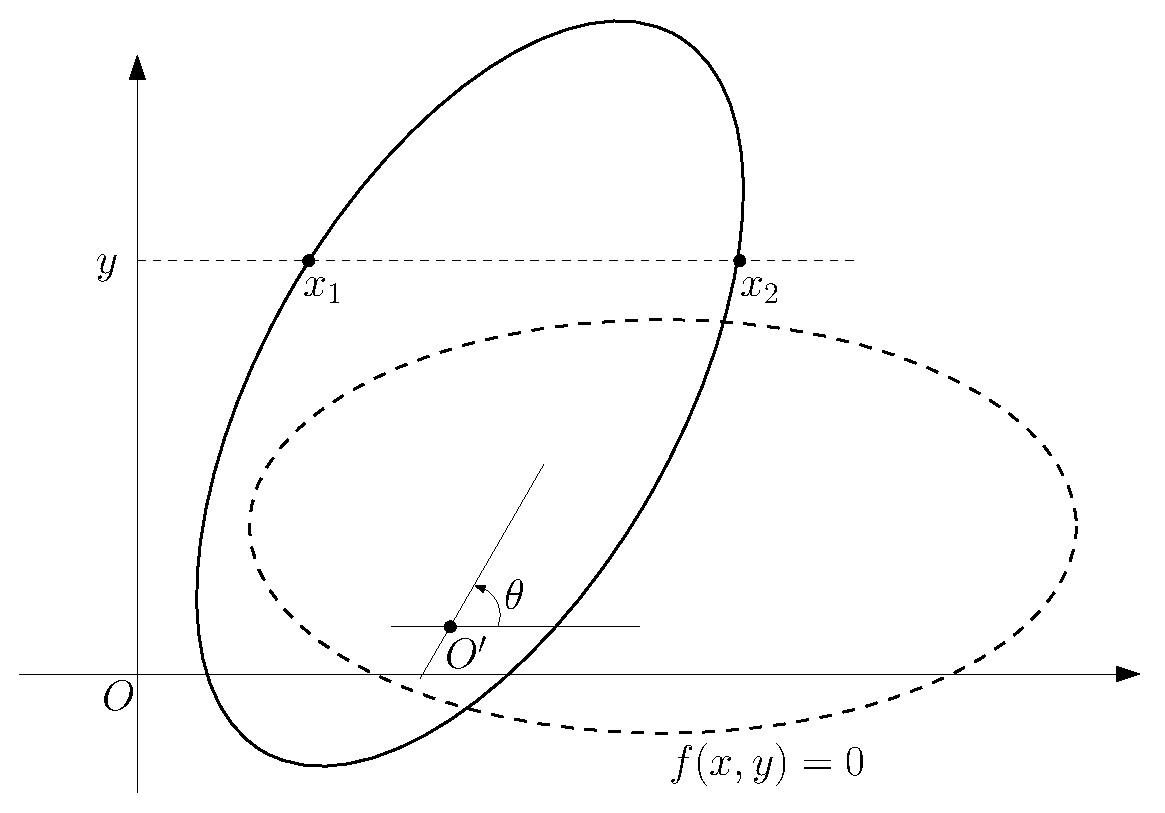
\includegraphics[width=0.6\textwidth]{transformation-1} \caption{Rotate transformation} \label{fig:1}
	%\includegraphics[width=0.4\textwidth]{hfaced-grid} \caption{H faced grid} \label{fig:10}
	%\includegraphics[width=0.4\textwidth]{hfaced-grid} \caption{E faced grid} \label{fig:10}
	%\subfigure[H faced grid]{\includegraphics[width=0.45\textwidth]{hfaced-grid} \label{fig:1a}}
	%\qquad
	%\subfigure[E faced grid]{\includegraphics[width=0.45\textwidth]{efaced-grid} \label{fig:1b}}
	%\caption{Rotate transformation}
	%\label{fig:1}
\end{figure}

\begin{framed}
	Q) $f(\mathbf{x})=0$을 만족하는 도형을 주어진 점 $\mathbf{O}'$을 기준으로 회전시켰다고 하자. 이 때 fdtd grid를 이루는 각 직선과의 교점은 어떻게 구할까?
\end{framed}

회전변환 하기 이전의 점들을 $\mathbf{x}_0$라 하면, $\mathbf{O}'$을 중심으로 회전변환 후의 점의 좌표는 다음과 같이 표현된다.
\begin{equation}
	\mathbf{x} = R(\theta)(\mathbf{x}_0-\mathbf{O}') + \mathbf{O}' \label{eq:1}
\end{equation}

\numberwithin{equation}{section}

\section{2 dimension}
Eq.(\ref{eq:1})을 매트릭스로 표현하면,
\begin{eqnarray}
	\left( \begin{array}{c}
		x \\ y
	\end{array}	\right)  
	&=& \left( \begin{array}{cc}
		\cos\theta & -\sin\theta \\
		\sin\theta & \cos\theta 
	\end{array}	\right)
	\left( \begin{array}{c}
		x_0 - O'_x \\
		y_0 - O'_y 
	\end{array}	\right) 
	+ \left( \begin{array}{c}
		O'_x \\
		O'_y 
	\end{array}	\right) \notag \\
	&=& \left( \begin{array}{c}
		\cos\theta(x_0 - O'_x) - \sin\theta(y_0 - O'_y) + O'_x \\
		\sin\theta(x_0 - O'_x) + \cos\theta(y_0 - O'_y) + O'_y 
	\end{array} \right) \label{eq:1.1}
\end{eqnarray}

\subsection{x가 주어지고 y를 구할 때,}
$f(x,y)=0$에서 $y_0=g_x(x_0)$을 알 수 있다면, Eq.(\ref{eq:1.1})에서 다음 2단계로 y를 구할 수 있다.\\

step 1) $h_x(x_0)=0$을 만족하는 $x_0$ 구하기
\begin{equation}
	h_x(x_0) = (x_0 - O'_x)\cos\theta - \left[g_x(x_0) - O'_y\right]\sin\theta + O'_x - x \label{eq:1.2}
\end{equation}

step 2) $x_0$을 대입하여 $y$ 구하기
\begin{equation}
	y = (x_0 - O'_x)\sin\theta + \left[g_x(x_0) - O'_y\right]\cos\theta + O'_y \label{eq:1.3}
\end{equation}

\subsection{y가 주어지고 x를 구할 때,}
마찬가지로 $x_0=g_y(y_0)$을 이용하여 x를 구할 수 있다.\\

step 1) $h_y(y_0)=0$을 만족하는 $y_0$ 구하기
\begin{equation}
	h_y(y_0) = \left[g_y(y_0) - O'_x\right]\sin\theta + (y_0 - O'_y)\cos\theta + O'_y - y \label{eq:1.4}
\end{equation}

step 2) $y_0$을 대입하여 $x$ 구하기
\begin{equation}
	x = \left[g_y(y_0) - O'_x\right]\cos\theta - (y_0 - O'_y)\sin\theta + O'_x \label{eq:1.5}
\end{equation}

\end{document}
